%\PassOptionsToPackage{draft}{graphicx}
\documentclass[aspectratio=169, 11pt]{beamer}%handout
\usepackage{fontspec}
\usetheme{metropolis}
\metroset{sectionpage=progressbar, progressbar=foot}
\setsansfont{Fira Sans Light}
\usepackage{appendixnumberbeamer}

\usepackage{booktabs}
\usepackage[scale=2]{ccicons}
\usepackage{multicol}

\usepackage{pgfplots}
\usepgfplotslibrary{dateplot}

\usepackage{xspace}
\newcommand{\themename}{\textbf{\textsc{metropolis}}\xspace}

\usepackage{hyperref}
%\usepackage[utf8]{inputenc}
%  % This line only for XeLaTeX and LuaLaTeX
\usepackage{pgfplots}

\graphicspath{{./images/}}

\title{Deep Gaussian Process for\\ Unsupervised Learning}
\subtitle{Semester project, Spring 2017 }
\date{\tiny\today}
\author{\textbf{Simone Rossi} \\ \vspace{0.5cm}Advisor Prof. Maurizio Filippone}
\institute{EURECOM, Ecole d'Ing\'enieur et Centre de Recherche en Telecommunications}
\titlegraphic{\hfill
\includegraphics[height=1.5cm]{logo.png}}

\begin{document}

\maketitle

\begin{frame}{Table of contents}
  \footnotesize
  \begin{multicols}{2}
        \footnotesize
        \setbeamertemplate{section in toc}[sections numbered]
        \setbeamertemplate{subsection in toc}[ball unnumbered]
        \tableofcontents[]%hideallsubsections
  \end{multicols}
\end{frame}

\definecolor{mygreen}{rgb}{0.2, 0.7, 0.2}
\definecolor{myorange}{rgb}{0.9, 0.5, 0.0}

\newcommand\noteMF[1]{\textcolor{red}{MF - #1}}
\newcommand\noteKC[1]{\textcolor{blue}{KC - #1}}
\newcommand\notePM[1]{\textcolor{mygreen}{PM - #1}}
\newcommand\noteSR[1]{\textcolor{myorange}{SR - #1}}

\newcommand{\nobs}{n} % Number of observations
\newcommand{\R}{\mathbb{R}}
\newcommand{\N}{\mathcal{N}}
%\newcommand{\C}{\mathbb{C}}
\newcommand{\Z}{\mathbb{Z}}
\newcommand{\F}{\mathcal{F}}
\newcommand{\I}{\mathcal{I}}
\newcommand{\LL}{\mathcal{L}}
% \newcommand{\vv}{\mathbf{v}}
\newcommand{\uu}{\mathbf{u}}
% \newcommand{\zz}{\mathbf{z}}
% \newcommand{\mm}{\mathbf{m}}
\newcommand{\ee}{\mathbf{e}}

% \newcommand{\KL}{\mathrm{KL}}
% \newcommand{\xnew}{x_{*}}
% \newcommand{\xvectnew}{\mathbf{x}_{*}}
% \newcommand{\tildexxnew}{\tilde{\mathbf{x}}_{*}}

%% \newcommand{\T}{\mathrm{T}}
\newcommand{\E}{\mathrm{E}}
\newcommand{\const}{\mathrm{const.}}
\newcommand{\diag}{\mathrm{diag}}
\newcommand{\Tr}{\mathrm{Tr}}
%% \newcommand{\vectorize}{\mathrm{vec}}


\newcommand{\norm}{\mathcal{N}}
%% \newcommand{\expdist}{\mathcal{E}}
%% \newcommand{\DP}{\mathcal{DP}}
%% \newcommand{\Beta}{\mathcal{B}}
%% \newcommand{\Ga}{\mathcal{G}}
%% \newcommand{\Wi}{\mathcal{W}}
%% \newcommand{\St}{\mathrm{St}}
%% \newcommand{\expfam}{\mathcal{E}}

\newcommand{\avect}{\mathbf{a}}
\newcommand{\dvect}{\mathbf{d}}
\newcommand{\fvect}{\mathbf{f}}
\newcommand{\gvect}{\mathbf{g}}
\newcommand{\Ivect}{\mathbf{I}}
\newcommand{\Kvect}{\mathbf{K}}
\newcommand{\hvect}{\mathbf{h}}
\newcommand{\Lvect}{\mathbf{L}}
\newcommand{\mvect}{\mathbf{m}}
\newcommand{\pvect}{\mathbf{p}}
\newcommand{\svect}{\mathbf{s}}
\newcommand{\uvect}{\mathbf{u}}
\newcommand{\Uvect}{\mathbf{U}}
\newcommand{\vvect}{\mathbf{v}}
\newcommand{\Vvect}{\mathbf{V}}
\newcommand{\zvect}{\mathbf{z}}
\newcommand{\xvect}{\mathbf{x}}
\newcommand{\Xvect}{\mathbf{X}}
\newcommand{\yvect}{\mathbf{y}}
\newcommand{\Yvect}{\mathbf{Y}}
\newcommand{\wvect}{\mathbf{w}}
\newcommand{\Wvect}{\mathbf{W}}
\newcommand{\tvect}{\mathbf{t}}
\newcommand{\zerovect}{\mathbf{0}}
\newcommand{\onesvect}{\mathbf{1}}

\newcommand{\Dobs}{D_\mathrm{obs}}
\newcommand{\Dlat}{D_\mathrm{lat}}

\newcommand{\betavect}{\boldsymbol{\beta}}
\newcommand{\thetavect}{\boldsymbol{\theta}}
\newcommand{\Thetavect}{\mathbf{\Theta}}
\newcommand{\psivect}{\boldsymbol{\psi}}
\newcommand{\Psivect}{\boldsymbol{\Psi}}
\newcommand{\Phivect}{\boldsymbol{\Phi}}
\newcommand{\Pivect}{\boldsymbol{\Pi}}
\newcommand{\etavect}{\boldsymbol{\eta}}
\newcommand{\rhovect}{\boldsymbol{\rho}}
\newcommand{\tauvect}{\boldsymbol{\tau}}
\newcommand{\nuvect}{\boldsymbol{\nu}}
\newcommand{\muvect}{\boldsymbol{\mu}}
\newcommand{\omegavect}{\boldsymbol{\omega}}
\newcommand{\Omegavect}{\mathbf{\Omega}}
\newcommand{\sigmavect}{\boldsymbol{\sigma}}
\newcommand{\zetavect}{\boldsymbol{\zeta}}
\newcommand{\varepsilonvect}{\boldsymbol{\epsilon}}
\newcommand{\deltavect}{\boldsymbol{\delta}}

\newcommand{\bigO}{\mathcal{O}}


\newcommand{\name}[1]{{\textsc{#1}}\xspace}

\newcommand{\mcmc}{\name{mcmc}}

% DATASETS
% Small
\newcommand{\cifar}{\name{cifar10}}
%% \newcommand{\rectangleshort}{\name{rect-img}}
%% \newcommand{\rectangle}{\name{rectangles-image}}
\newcommand{\mnisteight}{\textsc{mnist}8\textsc{m}\xspace}
%% \newcommand{\mining}{\name{mining}}
\newcommand{\protein}{\name{protein}}
\newcommand{\powerplant}{\name{powerplant}}
\newcommand{\spam}{\name{spam}}
\newcommand{\eeg}{\name{eeg}}
\newcommand{\usps}{\name{usps}}
% Medium
%% \newcommand{\sarcos}{\name{sarcos}} % sarcos all
\newcommand{\mnist}{\name{mnist}} % mnist all
%% \newcommand{\mnistbin}{\name{mnist-b}}
%% \newcommand{\sarcostwo}{\name{sarcos-2}}
% Large
\newcommand{\airline}{\name{airline}}

% Models
\newcommand{\autogp}{\textsc{a}uto\textsc{gp}\xspace}
\newcommand{\gpflow}{\textsc{gpf}low\xspace}
\newcommand{\tensorflow}{\textsc{T}ensor\textsc{F}low\xspace}

\newcommand{\arccosine}{\name{arc-cosine}}
\newcommand{\dbnthree}{\name{DBN}}
\newcommand{\svdkl}{\name{SV-DKL}}
\newcommand{\dgprbf}{\textsc{dgp}-\textsc{rbf}\xspace}
\newcommand{\dgparc}{\textsc{dgp}-\textsc{arc}\xspace}
\newcommand{\dgpep}{\textsc{dgp}-\textsc{ep}\xspace}
\newcommand{\dgpvar}{\textsc{dgp}-\textsc{var}\xspace}

\newcommand{\gplvm}{\name{gplvm}}
\newcommand{\dgplvm}{\name{dgplvm}}
\newcommand{\gp}{\name{gp}}
\newcommand{\gps}{\textsc{gp}s\xspace}
\newcommand{\dgp}{\name{dgp}}
\newcommand{\dgps}{\textsc{dgp}s\xspace}
\newcommand{\dnn}{\name{dnn}}
\newcommand{\dnns}{\textsc{dnn}s\xspace}
\newcommand{\svm}{\name{svm}}
\newcommand{\svms}{\textsc{svm}s\xspace}
\newcommand{\vargp}{\textsc{var}-\textsc{gp}\xspace}

\newcommand{\ard}{\name{ard}}
\newcommand{\softmax}{\name{softmax}}

\newcommand{\relu}{{\textsc{r}}e\name{lu}}

\newcommand{\arc}{\name{arc}}
\newcommand{\rbf}{\name{rbf}}

\newcommand{\adam}{\name{adam}}

% Metrics
\newcommand{\mnll}{\name{mnll}}
\newcommand{\rmse}{\name{rmse}}
\newcommand{\nelbo}{\name{nelbo}}

%!TEX root = dgplvm.tex

\section{Introduction}
\label{cap:introduction}

\subsection{Why unsupervised learning}
\begin{frame}{Why unsupervised learning}
    Unsupervised learning is more subjective than supervised learning, as there is no simple goal for the analysis. But techniques for unsupervised learning are of growing importance in a number of fields:
    \begin{itemize}
        \pause
        \item visualize and draw trends of high dimensional problems,
        \pause
        \item subgroups of breast cancer patients grouped by their gene expression measurements,
        \pause
        \item groups of shoppers characterized by their browsing and purchase histories,
        \item movies grouped by the ratings assigned by movie viewers.
    \end{itemize}
\end{frame}

\begin{frame}{Examples of unsupervised learning}
    \begin{minipage}{.48\textwidth}
        \begin{figure}
            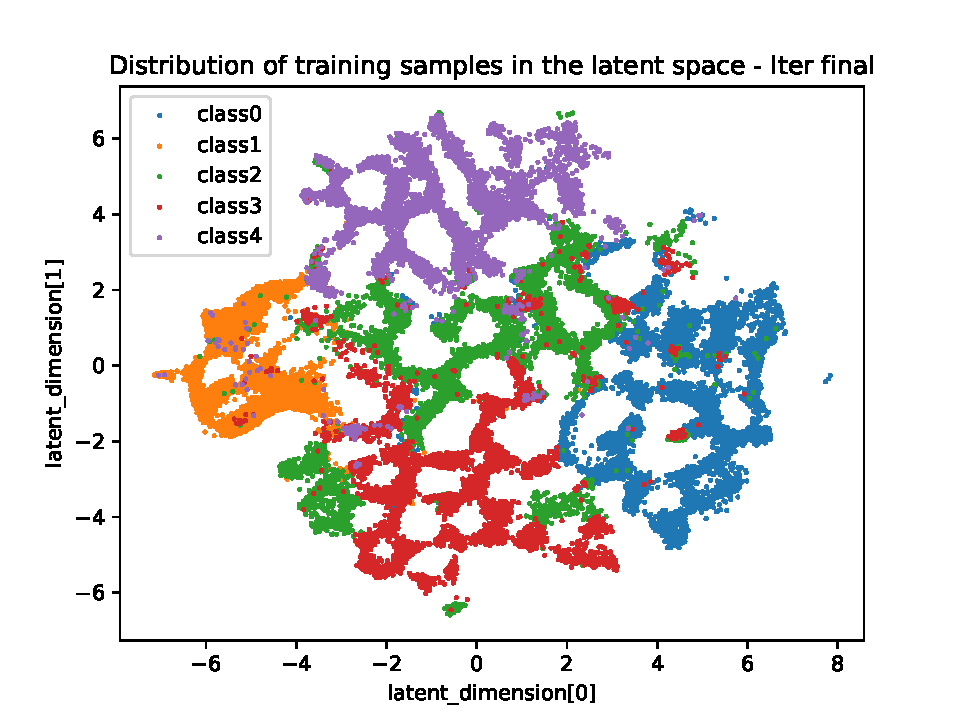
\includegraphics[width=\textwidth]{mnist_5classes_2dim.pdf}
            \caption{Feature projection of the \texttt{MNIST dataset} (5 digits)}
        \end{figure}
    \end{minipage}
    \begin{minipage}{.48\textwidth}
        \begin{figure}
            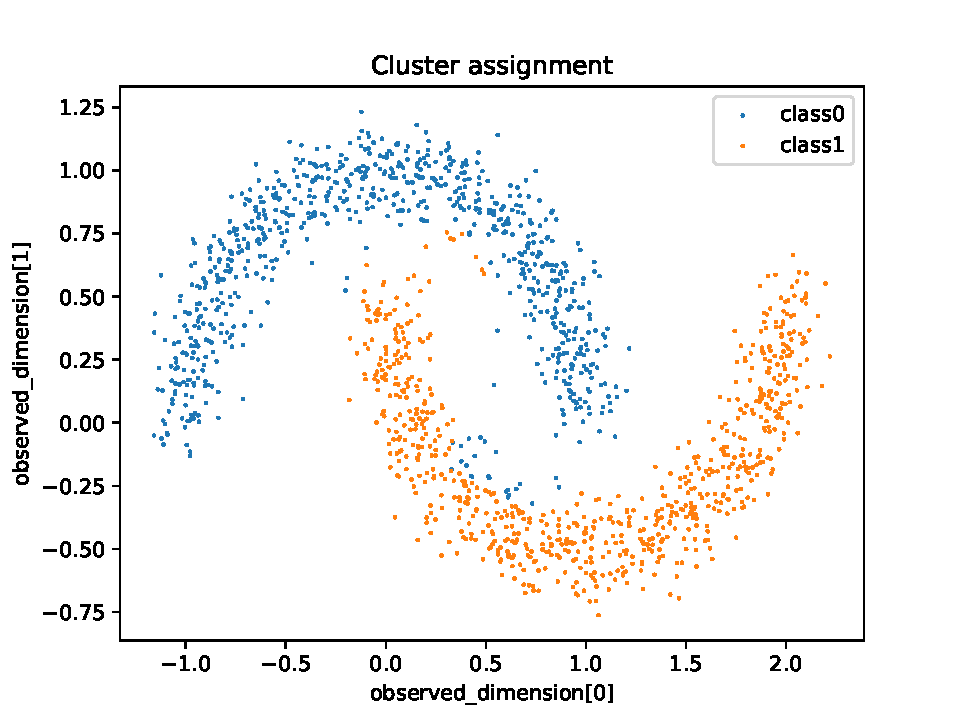
\includegraphics[width=\textwidth]{moons_assignment_cluster.pdf}
            \caption{Clustering assignment of the \texttt{sklearn} moon dataset}
        \end{figure}
    \end{minipage}
\end{frame}

%!TEX root = dgplvm.tex

\section{Deep Gaussian Processes}
\label{cap:dgp}

\subsection{Gaussian Process review}
\begin{frame}{Gaussian Process - Weight space}
    A Gaussian Process can be seen as a Bayesian linear regression with possibly infinite basis functions.
    \begin{equation}
        \bar f(\xvectnew) = \phi(\xvectnew)^\top\wvect.
    \end{equation}
    \pause
    Introducing the covariance function $k(\xvect, \xvect')$, it can be proved that the equation above can be written as follows
    \begin{equation}
        \bar f(\xvectnew) = \kvect(\xvectnew)^\top \alphavect,
    \end{equation}
    where $\alphavect = K^{-1}\yvect$ and $\kvect(\xvectnew)$ denote the vector of covariances between the point $\xvectnew$ and the $\nobs$ training points.
\end{frame}

\begin{frame}{Fourier expansion}
    The popular RBF kernel can be approximated as follows
    \begin{equation}
        k_{\mathrm{rbf}}(\xvect_i, \xvect_j) \approx \frac{1}{N_{\mathrm{RF}}} \sum_{r=1}^{N_{\mathrm{RF}}} \zvect(\xvect_i | \tilde{\omegavect}_r)^{\top} \zvect(\xvect_j | \tilde{\omegavect}_r) \text{,}
    \end{equation}
    where $\zvect(\xvect | \omegavect) = [\cos(\xvect^{\top} \omegavect), \sin(\xvect^{\top} \omegavect)]^{\top}$ and with $\tilde{\omegavect}_{r} \sim p(\omegavect)$.
\end{frame}

\subsection{Deep Architecture}
\begin{frame}{Deep Architecture}
    \def\layersep{1.4cm}
\def\scale{0.8}
\definecolor{myblue}{rgb}{0.2, 0.2, 0.8}
\newcommand{\red}{\textcolor{red}}
\newcommand{\orange}{\textcolor{orange}}
\newcommand{\green}{\textcolor{green}}
\newcommand{\blue}{\textcolor{blue}}
\newcommand\colorpar[1]{\textcolor{myyellow}{#1}}
\newcommand\colordata[1]{\textcolor{myorange}{#1}}
\newcommand\colorlatent[1]{\textcolor{myblue}{#1}}
\newcommand\colorweights[1]{\textcolor{mygreen}{#1}}

\begin{figure}[t]
\begin{tikzpicture}[shorten >=1pt,->,draw=green!50!black, node distance=\layersep]
    \tikzstyle{every pin edge}=[<-,shorten <=1pt]
    \tikzstyle{neuron}=[circle,minimum size=10pt,inner sep=0pt, draw=black]

    \tikzstyle{data neuron}=[neuron, fill=yellow!50!red];
    \tikzstyle{output neuron}=[neuron, fill=blue!50];
    \tikzstyle{hidden neuron}=[neuron];
    \tikzstyle{annot} = [text width=4em, text centered];
    \tikzstyle{annot-weight} = [text centered, fill=white!20, rectangle, draw];

    %% % Draw the input layer nodes
    %% \foreach \name / \y in {1,...,4}
    %%     \node[data neuron, pin=left:{\scriptsize $X$ \#\y}] (F0-\name) at (0,-\y) {};

    % Draw the input layer nodes
    \foreach \name / \y in {1,...,4}
        \node[data neuron] (F0-\name) at (0,\scale*-\y) {};

    % Draw the first hidden layer nodes - Phi^{(0)}
    \foreach \name / \y in {1,...,5}
        \path[yshift=\scale*0.5cm]
            node[hidden neuron] (Phi0-\name) at (\layersep,\scale*-\y cm) {};

    % Draw the layer node for F^{(1)}
    \foreach \name / \y in {1,...,2}
        \path[yshift=\scale*-1.0cm]
            node[output neuron] (F1-\name) at (2 * \layersep,\scale*-\y) {};

    % Draw the second hidden layer nodes - Phi^{(1)}
    \foreach \name / \y in {1,...,5}
        \path[yshift=\scale*0.5cm]
            node[hidden neuron] (Phi1-\name) at (3 * \layersep,\scale*-\y cm) {};

    % Draw the layer node for F^{(1)}
    \foreach \name / \y in {1,...,3}
        \path[yshift=\scale*-0.5cm]
            node[output neuron] (F2-\name) at (4 * \layersep,\scale*-\y) {};

    \foreach \name / \y in {1,...,3}
        \path[yshift=\scale*-0.5cm]
            node[data neuron] (Y-\name) at (5 * \layersep,\scale*-\y) {};

    % Draw Thetas
    \node[annot] (theta-0) at (0.5 * \layersep,\scale*-4.5) {\scriptsize\red{$\thetavect$}$^{(0)}$};
    \node[annot] (theta-1) at (2.5 * \layersep,\scale*-4.5) {\scriptsize\red{$\thetavect$}$^{(1)}$};


    %% \node[output neuron,pin={[pin edge={->}]right:{\scriptsize $F^{(1)}$}}, right of=Phi1-3] (F2) {};


    % Connect every node in the input layer with every node in the
    % hidden layer.
    \foreach \source in {1,...,4}
        \foreach \dest in {1,...,5}
            \path (F0-\source) edge (Phi0-\dest);

    % Connect every node in the hidden layer with the output layer
    \foreach \source in {1,...,5}
        \foreach \dest in {1,...,2}
            \path (Phi0-\source) edge (F1-\dest);

    % Connect every node in the hidden layer with the output layer
    \foreach \source in {1,...,2}
        \foreach \dest in {1,...,5}
            \path (F1-\source) edge (Phi1-\dest);

    % Connect every node in the hidden layer with the output layer
    \foreach \source in {1,...,5}
        \foreach \dest in {1,...,3}
            \path (Phi1-\source) edge (F2-\dest);

    % Connect every node in the hidden layer with the output layer
    \foreach \source in {1,...,3}
        \foreach \dest in {1,...,3}
            \path (F2-\source) edge (Y-\dest);

    % Annotate the layers
    \node[annot,above of=Phi0-1, node distance=0.6cm] (Layer-Phi0) {{\scriptsize $\Phi^{(0)}$}};
    \node[annot,left of=Layer-Phi0] {{\scriptsize $\colordata{X}$}};
    \node[annot,right of=Layer-Phi0] {{\scriptsize $\colorlatent{F}^{(1)}$}};
    \node[annot,above of=Phi1-1, node distance=0.6cm] (Layer-Phi1) {{\scriptsize $\Phi^{(1)}$}};
    \node[annot,right of=Layer-Phi1] {{\scriptsize $\colorlatent{F}^{(2)}$}};
    \node[annot,above of=Y-1, node distance=1.35cm] (Layer-Y) {{\scriptsize $\colordata{Y}$}};


    \node[annot-weight] (Omega-Phi0) at (0.5 * \layersep, \scale*-2.5) {{\scriptsize $\colorweights{\Omega}^{(0)}$}};
    \node[annot-weight,right of=Omega-Phi0] (W-Phi0) {{\scriptsize $\colorweights{W}^{(0)}$}};
    \node[annot-weight] (Omega-Phi1) at (2.5 * \layersep, \scale*-2.5) {{\scriptsize $\colorweights{\Omega}^{(1)}$}};
    \node[annot-weight,right of=Omega-Phi1] (W-Phi1) {{\scriptsize $\colorweights{W}^{(1)}$}};

    \path (theta-0) edge[red] (Omega-Phi0);
    \path (theta-1) edge[red] (Omega-Phi1);

\end{tikzpicture}
\caption{The \dgp approximation used for building the deep model. At each hidden layer \gp{s} are replaced by their two-layer weight-space approximation. Random-features $\Phi^{(l)}$ are obtained using a weight matrix $\Omega^{(l)}$. This is followed by a linear transformation parameterized by weights $W^{(l)}$. } 
\label{fig:DGP:diagram}
\end{figure}

    This is the approximation of \dgp where
    \begin{equation}
        \Phi_{\mathrm{rbf}}^{(l)} = \sqrt{\frac{(\sigma^2)^{(l)}}{N_{\mathrm{RF}}^{(l)}}} \left[ \cos\left(F^{(l)} \Omega^{(l)}\right), \sin\left(F^{(l)} \Omega^{(l)}\right) \right] \text{,}
    \end{equation}
    and
    \begin{equation}
        F^{(l+1)} = \Phi_{\mathrm{rbf}}^{(l)} W^{(l)} \text{.}
    \end{equation}
\end{frame}

%!TEX root = dgplvm.tex

\section{Latent Variable Models}
\label{cap:lvm}

\subsection{Probabilistic Principal Component Analysis}
\begin{frame}{Probabilistic Principal Component Analysis}
    One of the most important problems in unsupervised learning is to represent the observed data $\Yvect$ (with $\yvect_i \in R^{D_\mathrm{obs}}$) in some lower dimensional embedded space $\Xvect$ (with $\xvect_i \in R^{D_\mathrm{lat}}$), such that
    \begin{equation}
        \yvect_i = \Wvect\xvect_i + \varepsilon_i,
    \end{equation}
    where $\varepsilon_i \sim \N(0, \sigma^2\Ivect)$.\\
    \pause
    \vspace{0.5cm}
    The model is defined \textbf{probabilistically}, the latents are \textbf{marginalized} and the parameters are computed through \textbf{maximization}.\\
\end{frame}

\begin{frame}{Probabilistic Principal Component Analysis (cont.)}
    Let's define the likelihood as follows
    \begin{equation}
        p(\yvect_i\vert\xvect_i,\sigma^2) = \N(\Wvect\xvect_i, \sigma^2\Ivect)
    \end{equation}
    \pause
    We can now specify a simple prior over $\xvect_i$ and integrate out the latent variable
    \begin{equation}
        p(\yvect_i\vert\Wvect, \sigma^2) = \int p(\yvect_i\vert\xvect_i,\Wvect, \sigma^2) p(\xvect_i) d\xvect_i \pause = \N (\zerovect, \Wvect\Wvect^\top+\sigma^2\Ivect)
    \end{equation}
    \pause
    Thanks to point independence, the marginal likelihood on the whole dataset is
    \begin{equation}
        p(\Yvect\vert\Wvect, \sigma^2) = \prod_{i=0}^{\nobs-1} p(\yvect_i\vert\Wvect, \sigma^2)
    \end{equation}
    \pause
    Finally,
    \begin{equation}
        \Wvect = \arg\max_\Wvect p(\Yvect\vert\Wvect, \sigma^2)
    \end{equation}
\end{frame}

\subsection{Dual Probabilistic Principal Component Analysis}
\begin{frame}{Dual Probabilistic Principal Component Analysis}
    Differently, we can \textbf{marginalize} the parameters and compute the latents are computed through \textbf{maximization}. To do so, let's specify a prior over $\Wvect$:
    \begin{equation}
        p(\Wvect) = \prod_{i=0}^{\Dobs-1}\N(\wvect_i\vert\zerovect,\Ivect)
    \end{equation}
    \pause
    The marginal likelihood has the form
    \begin{equation}
        p(\Yvect\vert\Xvect, \sigma^2) = \prod_{i=0}^{\Dobs-1} \int p(\yvect_i\vert\xvect_i,\Wvect, \sigma^2) p(\Wvect) d\Wvect \pause = \prod_{i=0}^{\Dobs-1} \N(\yvect_{:,i}|\zerovect, \Xvect\Xvect^\top+\sigma^2\Ivect).
    \end{equation}
    \pause
    The corresponding loglikelihood is the following
    \begin{equation}
        \log p(\Yvect\vert\Xvect,\sigma^2) =  -\dfrac{\nobs\Dobs}{2}\ln(2\pi) - \dfrac{\Dobs}{2}\ln\vert\Kvect\vert - \dfrac{1}{2}\Tr\left(\Kvect^{-1}\Yvect\Yvect^\top\right)
    \end{equation}
\end{frame}

\begin{frame}{Dual Probabilistic Principal Component Analysis (cont.)}
    \begin{equation}
        \LL = \log p(\Yvect\vert\Xvect,\sigma^2) =  -\dfrac{\nobs\Dobs}{2}\ln(2\pi) - \dfrac{\Dobs}{2}\ln\vert\Kvect\vert - \dfrac{1}{2}\Tr\left(\Kvect^{-1}\Yvect\Yvect^\top\right)
    \end{equation}
    Since $\Kvect = \Xvect\Xvect^\top+\sigma^2\Ivect$, this is a product of $\Dobs$ independent Gaussian processes with linear covariance function.\\
    \pause
    The solution of the maximization problem is
    \begin{equation}
        \Xvect = \Uvect\Lvect\Vvect^\top
    \end{equation}
    where $\Uvect$ is an $\nobs\times\Dlat$ matrix whose columns are the first $\Dlat$ eigenvectors of $\Yvect\Yvect^\top$, $\Lvect$ is the associated diagonal eigenvalue matrix and $\Vvect$ is eventually a $\Dobs\times\Dobs$ rotation matrix.
\end{frame}

\subsection{Gaussian Process Latent Variable Model}
\begin{frame}{Gaussian Process Latent Variable Model}
    We can now replace the inner product kernel with a covariance function so that it allows non-linear transformation to obtain a non-linear latent variable model.
    \begin{equation}
        k_{\mathrm{rbf}}(\xvect_i, \xvect_j) = \exp\left[ -\dfrac{1}{2} \| \xvect_i-\xvect_j \|^2 \right]
    \end{equation}
    \pause
    Unfortunately there is not closed form solution of the maximization of the likelihood and therefore the resulting models will not be optimizable through an eigenvalue problem.
\end{frame}

%!TEX root = dgplvm.tex

\section{Clustering}

\subsection{From latents to cluster assignment}
\begin{frame}{From latents to cluster assignment}
    To actually making assignment to clusters, latents have to be discretized in order to give for each point a probability of being assigned to specific cluster.
    \pause
    \def\layersep{1.6cm}
\def\scale{0.8}
\definecolor{myblue}{rgb}{0.2, 0.2, 0.8}


\begin{figure}[t]
\begin{tikzpicture}[shorten >=1pt,->,draw=green!50!black, node distance=\layersep]
    \tikzstyle{every pin edge}=[<-,shorten <=1pt]
    \tikzstyle{neuron}=[circle,minimum size=10pt,inner sep=0pt, draw=black]

    \tikzstyle{data neuron}=[neuron, fill=yellow!50!red];
    \tikzstyle{output neuron}=[neuron, fill=blue!50];
    \tikzstyle{hidden neuron}=[neuron];
    \tikzstyle{annot} = [text width=4em, text centered];
    \tikzstyle{annot-weight} = [text centered, fill=white!20, rectangle, draw];

    %% % Draw the input layer nodes
    %% \foreach \name / \y in {1,...,4}
    %%     \node[data neuron, pin=left:{\scriptsize $X$ \#\y}] (F0-\name) at (0,-\y) {};

    % Draw the input layer nodes
    \foreach \name / \y in {1,...,4}
        \node[data neuron] (F0-\name) at (0,\scale*-\y) {};

    % Draw the first hidden layer nodes - Phi^{(0)}
    %\foreach \name / \y in {1,...,5}
    %    \path[yshift=\scale*0.5cm]
    %        node[hidden neuron] (Phi0-\name) at (\layersep,\scale*-\y cm) {};

    % Draw the layer node for F^{(1)}
    \foreach \name / \y in {1,...,4}
        \path[yshift=\scale]
            node[output neuron] (F1-\name) at (1 * \layersep,\scale*-\y) {};

    % Draw the second hidden layer nodes - Phi^{(1)}
    \foreach \name / \y in {1,...,5}
        \path[yshift=\scale*0.5cm]
            node[hidden neuron] (Phi1-\name) at (2 * \layersep,\scale*-\y cm) {};

    % Draw the layer node for F^{(1)}
    \foreach \name / \y in {1,...,3}
        \path[yshift=\scale*-0.5cm]
            node[output neuron] (F2-\name) at (3 * \layersep,\scale*-\y) {};

    \foreach \name / \y in {1,...,3}
        \path[yshift=\scale*-0.5cm]
            node[data neuron] (Y-\name) at (4 * \layersep,\scale*-\y) {};

    % Draw Thetas
    %\node[annot] (theta-0) at (0.5 * \layersep,\scale*-4.5) {\scriptsize\red{$\thetavect$}$^{(0)}$};
    %\node[annot] (theta-1) at (2.5 * \layersep,\scale*-4.5) {\scriptsize\red{$\thetavect$}$^{(1)}$};


    %% \node[output neuron,pin={[pin edge={->}]right:{\scriptsize $F^{(1)}$}}, right of=Phi1-3] (F2) {};


    % Connect every node in the input layer with every node in the
    % hidden layer.
    %\foreach \source in {1,...,4}
    %    \foreach \dest in {1,...,5}
    %        \path (F0-\source) edge (Phi0-\dest);

    % Connect every node in the hidden layer with the output layer
    \foreach \source in {1,...,4}
        \foreach \dest in {1,...,4}
            \path (F0-\source) edge (F1-\dest);

    % Connect every node in the hidden layer with the output layer
    \foreach \source in {1,...,4}
        \foreach \dest in {1,...,5}
            \path (F1-\source) edge (Phi1-\dest);

    % Connect every node in the hidden layer with the output layer
    \foreach \source in {1,...,5}
        \foreach \dest in {1,...,3}
            \path (Phi1-\source) edge (F2-\dest);

    % Connect every node in the hidden layer with the output layer
    \foreach \source in {1,...,3}
        \foreach \dest in {1,...,3}
            \path (F2-\source) edge (Y-\dest);

    % Annotate the layers
    \node[annot,above of=Phi0-1, node distance=0.6cm] (Layer-Phi0) {{\scriptsize $\colorlatent{\Pivect}$}};
    \node[annot,left of=Layer-Phi0] {{\scriptsize $\colordata{X}$}};
    %\node[annot,right of=Layer-Phi0] {{\scriptsize $\colorlatent{\Pivect}$}};
    \node[annot,above of=Phi1-1, node distance=0.6cm] (Layer-Phi1) {{\scriptsize $\Phi^{(1)}$}};
    \node[annot,right of=Layer-Phi1] {{\scriptsize $\colorlatent{F}^{(2)}$}};
    \node[annot,above of=Y-1, node distance=1.35cm] (Layer-Y) {{\scriptsize $\colordata{Y}$}};


    \node[annot-weight] (Omega-Phi0) at (0.5 * \layersep, \scale*-2.5) {{\scriptsize $\colorweights{\softmax}$}};
    %\node[annot-weight,right of=Omega-Phi0] (W-Phi0) {{\scriptsize $\colorweights{W}^{(0)}$}};
    \node[annot-weight] (Omega-Phi1) at (1.5 * \layersep, \scale*-2.5) {{\scriptsize $\colorweights{\Omega}^{(1)}$}};
    \node[annot-weight,right of=Omega-Phi1] (W-Phi1) {{\scriptsize $\colorweights{W}^{(1)}$}};

    %\path (theta-0) edge[red] (Omega-Phi0);
    %\path (theta-1) edge[red] (Omega-Phi1);

\end{tikzpicture}
\caption{The \dgp approximation used for building the deep model. At each hidden layer \gp{s} are replaced by their two-layer weight-space approximation. Random-features $\Phi^{(l)}$ are obtained using a weight matrix $\Omega^{(l)}$. This is followed by a linear transformation parameterized by weights $W^{(l)}$. }
\label{fig:DGP:diagram}
\end{figure}

\end{frame}

\begin{frame}{From latents to cluster assignment (cont.)}
    \def\layersep{1.6cm}
\def\scale{0.8}
\definecolor{myblue}{rgb}{0.2, 0.2, 0.8}


\begin{figure}[t]
\begin{tikzpicture}[shorten >=1pt,->,draw=green!50!black, node distance=\layersep]
    \tikzstyle{every pin edge}=[<-,shorten <=1pt]
    \tikzstyle{neuron}=[circle,minimum size=10pt,inner sep=0pt, draw=black]

    \tikzstyle{data neuron}=[neuron, fill=yellow!50!red];
    \tikzstyle{output neuron}=[neuron, fill=blue!50];
    \tikzstyle{hidden neuron}=[neuron];
    \tikzstyle{annot} = [text width=4em, text centered];
    \tikzstyle{annot-weight} = [text centered, fill=white!20, rectangle, draw];

    %% % Draw the input layer nodes
    %% \foreach \name / \y in {1,...,4}
    %%     \node[data neuron, pin=left:{\scriptsize $X$ \#\y}] (F0-\name) at (0,-\y) {};

    % Draw the input layer nodes
    \foreach \name / \y in {1,...,4}
        \node[data neuron] (F0-\name) at (0,\scale*-\y) {};

    % Draw the first hidden layer nodes - Phi^{(0)}
    %\foreach \name / \y in {1,...,5}
    %    \path[yshift=\scale*0.5cm]
    %        node[hidden neuron] (Phi0-\name) at (\layersep,\scale*-\y cm) {};

    % Draw the layer node for F^{(1)}
    \foreach \name / \y in {1,...,4}
        \path[yshift=\scale]
            node[output neuron] (F1-\name) at (1 * \layersep,\scale*-\y) {};

    % Draw the second hidden layer nodes - Phi^{(1)}
    \foreach \name / \y in {1,...,5}
        \path[yshift=\scale*0.5cm]
            node[hidden neuron] (Phi1-\name) at (2 * \layersep,\scale*-\y cm) {};

    % Draw the layer node for F^{(1)}
    \foreach \name / \y in {1,...,3}
        \path[yshift=\scale*-0.5cm]
            node[output neuron] (F2-\name) at (3 * \layersep,\scale*-\y) {};

    \foreach \name / \y in {1,...,3}
        \path[yshift=\scale*-0.5cm]
            node[data neuron] (Y-\name) at (4 * \layersep,\scale*-\y) {};

    % Draw Thetas
    %\node[annot] (theta-0) at (0.5 * \layersep,\scale*-4.5) {\scriptsize\red{$\thetavect$}$^{(0)}$};
    %\node[annot] (theta-1) at (2.5 * \layersep,\scale*-4.5) {\scriptsize\red{$\thetavect$}$^{(1)}$};


    %% \node[output neuron,pin={[pin edge={->}]right:{\scriptsize $F^{(1)}$}}, right of=Phi1-3] (F2) {};


    % Connect every node in the input layer with every node in the
    % hidden layer.
    %\foreach \source in {1,...,4}
    %    \foreach \dest in {1,...,5}
    %        \path (F0-\source) edge (Phi0-\dest);

    % Connect every node in the hidden layer with the output layer
    \foreach \source in {1,...,4}
        \foreach \dest in {1,...,4}
            \path (F0-\source) edge (F1-\dest);

    % Connect every node in the hidden layer with the output layer
    \foreach \source in {1,...,4}
        \foreach \dest in {1,...,5}
            \path (F1-\source) edge (Phi1-\dest);

    % Connect every node in the hidden layer with the output layer
    \foreach \source in {1,...,5}
        \foreach \dest in {1,...,3}
            \path (Phi1-\source) edge (F2-\dest);

    % Connect every node in the hidden layer with the output layer
    \foreach \source in {1,...,3}
        \foreach \dest in {1,...,3}
            \path (F2-\source) edge (Y-\dest);

    % Annotate the layers
    \node[annot,above of=Phi0-1, node distance=0.6cm] (Layer-Phi0) {{\scriptsize $\colorlatent{\Pivect}$}};
    \node[annot,left of=Layer-Phi0] {{\scriptsize $\colordata{X}$}};
    %\node[annot,right of=Layer-Phi0] {{\scriptsize $\colorlatent{\Pivect}$}};
    \node[annot,above of=Phi1-1, node distance=0.6cm] (Layer-Phi1) {{\scriptsize $\Phi^{(1)}$}};
    \node[annot,right of=Layer-Phi1] {{\scriptsize $\colorlatent{F}^{(2)}$}};
    \node[annot,above of=Y-1, node distance=1.35cm] (Layer-Y) {{\scriptsize $\colordata{Y}$}};


    \node[annot-weight] (Omega-Phi0) at (0.5 * \layersep, \scale*-2.5) {{\scriptsize $\colorweights{\softmax}$}};
    %\node[annot-weight,right of=Omega-Phi0] (W-Phi0) {{\scriptsize $\colorweights{W}^{(0)}$}};
    \node[annot-weight] (Omega-Phi1) at (1.5 * \layersep, \scale*-2.5) {{\scriptsize $\colorweights{\Omega}^{(1)}$}};
    \node[annot-weight,right of=Omega-Phi1] (W-Phi1) {{\scriptsize $\colorweights{W}^{(1)}$}};

    %\path (theta-0) edge[red] (Omega-Phi0);
    %\path (theta-1) edge[red] (Omega-Phi1);

\end{tikzpicture}
\caption{The \dgp approximation used for building the deep model. At each hidden layer \gp{s} are replaced by their two-layer weight-space approximation. Random-features $\Phi^{(l)}$ are obtained using a weight matrix $\Omega^{(l)}$. This is followed by a linear transformation parameterized by weights $W^{(l)}$. }
\label{fig:DGP:diagram}
\end{figure}

    \pause
    The \softmax layer simply implements a softmax function on each samples of the latent space $\Xvect$; in practice:
    \begin{equation}
        \Pivect = \dfrac{\exp(\Xvect)} {\sum_{j=0}^{D\mathrm{lat} - 1} \exp(\Xvect_{:,j})}
    \end{equation}

\end{frame}

%!TEX root = report.tex

\section{Experiments}

TODO

\subsection{Dimensionality reduction for visualisation}

TODO

\subsubsection{Latents initialization}

TODO

\subsection{Clustering}

TODO

\section{Conclusions}

In this work, we have proposed a novel formulation of \dgp{s} which exploits the approximation of covariance functions using random features, as well as stochastic variational inference for preserving the probabilistic representation of a regular \gp.
We demonstrated how inference using this model is not only faster, but also frequently superior to other state-of-the-art methods, with particular emphasis on competing \dgp models.
The results obtained for both the \airline dataset and the \mnisteight digit recognition problem are particularly impressive since such large datasets have been generally considered to be beyond the computational scope of \dgp{s}.
We perceive this to be a considerable step forward in the direction of scaling and accelerating \dgp{s}.

The results obtained on higher-dimensional datasets strongly suggest that approximations such as Fastfood~\cite{Smola13} could be instrumental in the interest of using more random features.
We are also currently investigating ways to mitigate the decline in performance observed when optimizing $\Omegavect$ variationally with resampling. 
The obtained results also encourage the extension of our model to include residual learning or convolutional layers suitable for computer vision applications.

%\begin{frame}[plain]
  \begin{tikzpicture}[remember picture,overlay]
    \node[at=(current page.center)] {
      \includegraphics[width=\paperwidth]{crowd_street.jpg}
    };
  \end{tikzpicture}
\end{frame}

\section{Partial Occlusion Handling}
\label{sec:Partial Occlusion Handling}


\begin{frame}{Partial Occlusion Handling}
\small
\metroset{block=fill}

  \begin{alertblock}{\textbf{Why?}}
  Generally, especially in crowded scenes, occlusions occur frequently.
  Nevertheless, generic detectors, such as HOG, assume that pedestrians are fully
  visible and their performance degrades when pedestrians are partially occluded.
  \end{alertblock}
\pause

  \begin{exampleblock}{\textbf{How?}}
  The key to successful detection of partially occluded pedestrians is to use additional
  information about which body parts are occluded, for example \textit{correlations among
  the visibilities of different parts} having different sizes.
  \end{exampleblock}

\end{frame}


\begin{frame}{Partial Occlusion Handling}
  \metroset{block=fill}
  \begin{alertblock}{Probabilistic Framework}
    It models correlations among the visibilities of parts as hidden variables
  \end{alertblock}

\pause

  \begin{exampleblock}{Deep Model}
    The hierarchical structure of the deep model matches with the multilayers of
    the parts model well.
    Different from the other types of deep networks, whose hidden variables had
    no semantic meaning, this model considers each hidden variable as representing
    the visibility of a part.
  \end{exampleblock}

\end{frame}


\begin{frame}{Hidden variable framework}
\small
Let $\mathbf{x}\in\mathbb{R}^d$ and $y\in\lbrace0,1\rbrace$ be respectively the \textit{feature vector} and the \textit{label} of a detection window.\\
\vspace{3mm}
Denote the detection scores of the $P$ parts by $\mathbf{s} = [s_1,...,s_P]^T = \gamma(\mathbf{x})$, where $\gamma(\mathbf{x})$ are part detectors.\\
\vspace{3mm}
Denote the visibilities of the $P$ parts by $\mathbf{h} = [h_1,...,h_P]^T \in\lbrace0,1\rbrace^P$, with $h_i = 1$ meaning \textbf{visible} and $h_i = 0$ meaning \textbf{invisible}.
\begin{equation}
  p(y\vert\mathbf{x}) = \sum_\mathbf{h}p(y,\mathbf{h}\vert\mathbf{x}) = \sum_\mathbf{h}p(y\vert\mathbf{h},\mathbf{x})p(\mathbf{h}\vert\mathbf{x})
\end{equation}

\end{frame}



%\pause
%  Often, for a fast approximate solution, this relation is simplified as follows:
%\begin{equation}
%  p(y\vert\mathbf{x}) \approx \exp \left( \sum_i s_i \right)
%\end{equation}

%\pause
%\metroset{block=fill}
%\begin{block}{Objective}
%  Build a deep model that learns the correlation of visibility
%   relationship among parts
%\end{block}

%\end{frame}

\begin{frame}{Deep Model for Part Visibility Estimation}
  \small
  \metroset{block=fill}
  \begin{block}{Objective}
    Build a deep model that learns the correlation of visibility
     relationship among parts
  \end{block}
  \pause
\centering
\includegraphics[width=0.85\textwidth]{mlp2.png}
\\
%\includegraphics[width=0.3\textwidth]{mlp1.png}
\end{frame}

\begin{frame}{Result}
  \includegraphics[width=\textwidth]{mlp_result.png}
\end{frame}


%\input{chapters/cnn.tex}



\end{document}
%
